\documentclass{article}

% Language setting
% Replace `english' with e.g. `spanish' to change the document language
\usepackage[english]{babel}
\usepackage{listings}
\usepackage{xcolor}
\usepackage{minted}

\lstset{ 
  backgroundcolor=\color{white},   % choose the background color; you must add \usepackage{color} or \usepackage{xcolor}; should come as last argument
  basicstyle=\footnotesize,        % the size of the fonts that are used for the code
  breakatwhitespace=false,         % sets if automatic breaks should only happen at whitespace
  breaklines=true,                 % sets automatic line breaking
  captionpos=b,                    % sets the caption-position to bottom
  commentstyle=\color{mygreen},    % comment style
  deletekeywords={...},            % if you want to delete keywords from the given language
  escapeinside={\%*}{*)},          % if you want to add LaTeX within your code
  extendedchars=true,              % lets you use non-ASCII characters; for 8-bits encodings only, does not work with UTF-8
  firstnumber=1000,                % start line enumeration with line 1000
  frame=single,	                   % adds a frame around the code
  keepspaces=true,                 % keeps spaces in text, useful for keeping indentation of code (possibly needs columns=flexible)
  keywordstyle=\color{blue},       % keyword style
  language=Octave,                 % the language of the code
  morekeywords={*,...},            % if you want to add more keywords to the set
  numbers=left,                    % where to put the line-numbers; possible values are (none, left, right)
  numbersep=5pt,                   % how far the line-numbers are from the code
  numberstyle=\tiny\color{mygray}, % the style that is used for the line-numbers
  rulecolor=\color{black},         % if not set, the frame-color may be changed on line-breaks within not-black text (e.g. comments (green here))
  showspaces=false,                % show spaces everywhere adding particular underscores; it overrides 'showstringspaces'
  showstringspaces=false,          % underline spaces within strings only
  showtabs=false,                  % show tabs within strings adding particular underscores
  stepnumber=2,                    % the step between two line-numbers. If it's 1, each line will be numbered
  stringstyle=\color{mymauve},     % string literal style
  tabsize=2,	                   % sets default tabsize to 2 spaces
  title=\lstname                   % show the filename of files included with \lstinputlisting; also try caption instead of title
}


\usepackage[letterpaper,top=2cm,bottom=2cm,left=3cm,right=3cm,marginparwidth=1.75cm]{geometry}

% Useful packages
\usepackage{amsmath}
\usepackage{graphicx}
\usepackage[colorlinks=true, allcolors=blue]{hyperref}
\usepackage{subfig}

\title{Projet Reseau}
\author{Nathan Seignole Mathis Vermeren}

\begin{document}
\maketitle

\section{Introduction}
Ce code est un systeme bancaire fonctionnant en TCP et UDP, en mutli-clients. Voici comment l'utiliser : 
Faire "make" dans ./UDP ou ./TCP
\newline
Lancer le server avec :
\newline
./server.out localhost PORT
\newline
\newline
Lancer le client avec : 
\newline
./client.out localhost PORT username
\newline
\newline
Les comptes déjà créés s'affichent en console : 
\newline
 - Un utilisateur avec pour ID : 1 et mot de passe : chaton123
\newline
 - Deux comptes 101 et 102.
\newline
(changer dans le main.c en cas de besoins).
\newline
On peut quitter le programme avec exit.

\section{Gestionnaire de base de données (bank.c, structBank.h)}

La base de données bancaire est définie dans le fichier \texttt{structBank.h}. Les différentes structures utilisées sont les suivantes :

\begin{minted}{c}
typedef enum Operation_type{
    AJOUT,
    RETRAIT
} Operation_t;

typedef struct Operation
{
    char date[64];
    Operation_t type;
    float somme;
} Operation;

typedef struct {
    int account_id;
    float balance;
    Operation operations[MAX_OPERATIONS];
    int num_operations;
} Account;

typedef struct {
   SOCKET sock;
   char name[BUF_SIZE];
} Client;

typedef struct {
   int user_id;
   char password[MAX_PASSWORD_LENGTH];
   Account accounts[MAX_ACCOUNTS];
   int num_accounts;
} User;
\end{minted}


La partie \mintinline{c}{bank.c} est identique en UDP et en TCP et réalise une interface entre le serveur et sa base de données. Les fonctions suivantes sont disponibles :

\mintinline{c}{void initialize_user(User *users, int user_id, const char *password)} : Ajoute un utilisateur.\newline
\mintinline{c}{void add_account(User *users, int user_id, int account_id, const char *password)} : Ajoute un compte à un utilisateur.

Les quatre commandes (ajout, retrait, solde, opérations) ont chacune leur fonction respective prenant comme argument le tableau \mintinline{c}{User *users}, qui représente la base de données.

Il existe également une fonction \mintinline{c}{add_operation} qui, entre autres, prend un \mintinline{c}{Operation_t} (AJOUT ou RETRAIT) en argument pour l'ajouter à l'historique des opérations, représenté par le tableau \mintinline{c}{Operation operations[MAX_OPERATIONS]}.

Enfin, le fichier \mintinline{c}{server.c} utilise uniquement la fonction : \newline
 \mintinline{c}{void process_command(User *users, char *buffer, char *res)}, qui prend la commande saisie par le client en entrée, la redirige vers la bonne fonction, et renvoie dans \mintinline{c}{res} un résultat ou une erreur.
\newline
Voici le corps de la fonction \mintinline{c}{process_command} : 
\begin{minted}{c}
void process_command(User *users,  char *buffer, char *res) {
    char command[20];
    int user_id, id_compte;
    char password[MAX_PASSWORD_LENGTH];
    double somme = 0.0; 
    int result = sscanf(buffer, "%s %d %d %s %lf", command, &user_id, &id_compte, password, &somme);
    printf("Scanned : %s %d %d %s %f\n",command, user_id, id_compte, password, somme);
    printf("Command : %s\n",command);
    if (result < 3) {
        strncpy(res,"KO : Le format de la commande est invalide",255);
    } 
    if (strcmp(command, "AJOUT") == 0 || strcmp(command, "RETRAIT") == 0) {
        if (result < 5) {
            strncpy(res,"KO : Pas suffisamment d'arguments pour AJOUT ou RETRAIT",255);
        }
    }
    // Traiter la commande en fonction du type
    if (strcmp(command, "AJOUT") == 0) {
        ajout(users, user_id, id_compte, password, res, somme);
    } else if (strcmp(command, "RETRAIT") == 0) {
        retrait(users, user_id, id_compte, password, res, somme);
    } else if (strcmp(command, "SOLDE") == 0) {
        solde(users, user_id, id_compte, password, res);
    } else if (strcmp(command, "OPERATIONS") == 0) {
        operations(users, user_id, id_compte, password, res);
    } else {
        strncpy(res,"KO : Commande inconnue",255);
    }
    printf("Response : %s\n",res);
    
    return;
}
\end{minted}


\section{Mise en place de la communication réseau}

\subsection{Initialisation de la connnexion côté serveur}
Que ça soit en UDP ou TCP, le programme commence par une fonction \mintinline{c}{void init(void)} qui nous sert juste à rendre le code compatible avec windows avec : \mintinline{c}{WSAStartup(MAKEWORD(2, 2), &wsa);}. Elle permet d'initialiser une DLL permettant d'utiliser les sockets. Pareillement, \mintinline{c}{void end(void)} permet de libérer cette même DLL avec \mintinline{c}{WSACleanup();}.

On entre ensuite dans \mintinline{c}{int init_connection(int PORT)}, elle crée un socket, configure son adresse et son port, le lie à l'adresse et au port spécifiés, puis le met en mode écoute (seulement en TCP) pour accepter les connexions entrantes.
On créer le socket : 

\begin{minted}{c}
   SOCKET sock = socket(AF_INET, SOCK_STREAM, 0);
\end{minted}
On utilise un protocoles internet IPV4 (AF\_INET), SOCK\_STREAM est un type de communication TPC, on utilise SOCK\_DGRAM en UDP, et 0 correspond au protocol par défaut. 

La structure \mintinline{c}{sockaddr_in} (sin) est configurée pour spécifier l'adresse IP et le port auquel le serveur sera lié.

Configuration de la Structure \mintinline{c}{sockaddr_in} :

\begin{minted}{c}
   sin.sin_addr.s_addr = htonl(INADDR_ANY);
   sin.sin_port = htons(PORT);
   sin.sin_family = AF_INET;
\end{minted}

\mintinline{c}{sin.sin_addr.s_addr} : L'adresse IP est configurée en utilisant \mintinline{c}{htonl} pour convertir l'adresse IP en format réseau.
\newline
\mintinline{c}{sin.sin_port} : Le numéro de port est configuré en utilisant \mintinline{c}{htons} pour convertir le numéro de port en format réseau.
\newline
\mintinline{c}{sin.sin_family} : La famille d'adresses est spécifiée comme étant IPv4.

\subsubsection*{Liaison du Socket}

\begin{minted}{c}
   bind(sock, (SOCKADDR *) &sin, sizeof sin);
\end{minted}

Cette étape associe une adresse IP et un numéro de port au socket créé.

\subsubsection*{Mise en Mode Écoute (TCP)}

\begin{minted}{c}
   listen(sock, MAX_CLIENTS);
\end{minted}

Le socket est mis en mode écoute pour accepter les connexions entrantes, avec \mintinline{c}{MAX_CLIENTS} spécifiant le nombre maximal de connexions en attente dans la file d'attente.

\subsection{Fonctions clés de la communication réseau : }


La fonction \mintinline{c}{accept} est utilisée pour accepter une nouvelle connexion TCP. Elle prend le socket d'écoute (\mintinline{c}{sock}), crée un nouveau socket dédié à la communication avec le client (\mintinline{c}{csock}), et récupère les informations du client telles que son adresse IP et le port utilisé.

\begin{minted}{c}
int csock = accept(sock, (SOCKADDR *)&csin, &sinsize);
\end{minted}

La fonction \mintinline{c}{send} est utilisée pour envoyer des données sur un socket TCP. Elle prend en argument le descripteur de socket (\mintinline{c}{sock}), le tampon contenant les données (\mintinline{c}{buffer}), la longueur des données à envoyer (\mintinline{c}{length}), et des options supplémentaires (\mintinline{c}{flags}).

\begin{minted}{c}
send(sock, buffer, length, flags);
\end{minted}

La fonction \mintinline{c}{sendto} est utilisée pour envoyer des données sur un socket UDP avec spécification du destinataire. Elle prend en argument le descripteur de socket (\mintinline{c}{sock}), le tampon contenant les données (\mintinline{c}{buffer}), la longueur des données à envoyer (\mintinline{c}{length}), des options supplémentaires (\mintinline{c}{flags}), et les informations sur le destinataire (\mintinline{c}{to}).

\begin{minted}{c}
sendto(sock, buffer, length, flags, (SOCKADDR *)&to, sizeof to);
\end{minted}

La fonction \mintinline{c}{recv} est utilisée pour recevoir des données depuis un socket TCP. Elle prend en argument le descripteur de socket (\mintinline{c}{sock}), le tampon où stocker les données reçues (\mintinline{c}{buffer}), la longueur maximale des données à recevoir (\mintinline{c}{length}), et des options supplémentaires (\mintinline{c}{flags}).

\begin{minted}{c}
recv(sock, buffer, length, flags);
\end{minted}

La fonction \mintinline{c}{recvfrom} est utilisée pour recevoir des données depuis un socket UDP avec spécification de l'expéditeur. Elle prend en argument le descripteur de socket (\mintinline{c}{sock}), le tampon où stocker les données reçues (\mintinline{c}{buffer}), la longueur maximale des données à recevoir (\mintinline{c}{length}), des options supplémentaires (\mintinline{c}{flags}), et les informations sur l'expéditeur (\mintinline{c}{from}).

\begin{minted}{c}
recvfrom(sock, buffer, length, flags, (SOCKADDR *)&from, &fromlen);
\end{minted}


\subsubsection{Gestion des Entrées/Sorties dans un Serveur TCP}

Pour gérer les entrées/sorties (E/S) dans un serveur TCP, la fonction \mintinline{c}{select} et les macros \mintinline{c}{FD_SET} et \mintinline{c}{FD_ISSET} sont couramment utilisées.

La fonction \mintinline{c}{FD_SET} permet d'ajouter des descripteurs de fichiers à un ensemble. Dans le contexte d'un serveur, on peut ajouter le descripteur du clavier (\mintinline{c}{STDIN_FILENO}) et le descripteur du socket (\mintinline{c}{sock}) à l'ensemble \mintinline{c}{rdfs}.

\begin{minted}{c}
FD_SET(STDIN_FILENO, &rdfs);
FD_SET(sock, &rdfs);
\end{minted}

La fonction \mintinline{c}{select} permet d'attendre que l'un des descripteurs de fichiers spécifiés soit prêt en lecture ou en écriture. Elle prend en compte trois ensembles : \mintinline{c}{readfds}, \mintinline{c}{writefds}, et \mintinline{c}{exceptfds}. Dans le contexte du serveur, on s'intéresse principalement à \mintinline{c}{readfds}, donc \mintinline{c}{select} surveille les descripteurs en lecture.

\begin{minted}{c}
select(sock + 1, &rdfs, NULL, NULL, NULL);
\end{minted}

La macro \mintinline{c}{FD_ISSET} permet de tester si un descripteur de fichier spécifique est prêt en lecture ou en écriture dans un ensemble donné. Dans le contexte du serveur, on teste si l'activité provient du clavier (\mintinline{c}{STDIN_FILENO}) ou du socket (\mintinline{c}{sock}).

\begin{minted}{c}
if (FD_ISSET(STDIN_FILENO, &rdfs)) {
    // Activité sur le clavier
}

if (FD_ISSET(sock, &rdfs)) {
    // Activité sur le socket
}
\end{minted}

Lorsqu'un nouveau client se connecte, son descripteur de socket (\mintinline{c}{csock}) peut être ajouté à l'ensemble \texttt{rdfs} pour surveiller son activité.

\begin{minted}{c}
FD_SET(csock, &rdfs);
\end{minted}

Cela permet de détecter si le client envoie des données.







\subsection{Différence entre l'UDP et le TCP}
UDP n'utilisant pas de connexion, on ne trouvera de fonction \mintinline{c}{listen} ou \mintinline{c}{accept}. Cependant, on ne peut plus utiliser les fonctions \mintinline{c}{send} ou \mintinline{c}{recv}. Dans notre base de données server, on ne stocke plus les descripteurs de socket des clients (\mintinline{c}{SOCKET} dans le code) mais leurs \mintinline{c}{SOCKADDR_IN}, qui des IP et des ports. C'est pourquoi il a fallu modifier une ligne de notre \mintinline{c}{structBank.h}, qui devient :

\begin{minted}{c}
typedef struct {
   SOCKADDR_IN sin;
   char name[BUF_SIZE];
} Client;
\end{minted}

On utilise alors d'autres fonctions d'envoie et de reception qui prennent SOCKADDR\_IN qui sont \mintinline{c}{sendto} ou \mintinline{c}{recvfrom}.

\subsection{Communication reseau côté Client }

L'initialisation de la communication est quasiment la même que côté serveur. 
Voici la fonction qui permet de lire et d'envoyer des commandes au serveur.
\begin{minted}{c}
void command_input(SOCKET sock){
   char input[256];
   printf("Enter a command : ");
   memset(input,0,256);
   fgets(input,255,stdin);

   //exit command
   if(!strcmp(input, "exit\n"))
     return;
   write_server(sock, input);
   memset(input,0,256);
   read_server(sock, input);
   printf("Read : %s\n", input);
}
\end{minted}

Command\_input est mis dans une boucle \mintinline{c}{while(1)} où on écoute les entrées clavier avec \newline \mintinline{c}{FD_ISSET(STDIN_FILENO, &rdfs)} ou les paquets arrivant avec  \mintinline{c}{FD_ISSET(sock, &rdfs)}. Cette fonction est la même en TCP et UDP. Comme côté Client on n'accepte pas de connexion et on n'écoute pas de port, on n'utilise ni accept, ni listen et seules les fonctions \mintinline{c}{wirte_client}, \mintinline{c}{read_client} , et le protocole de communication à l'initialisation de la socket (SOCK\_DGRAM et SOCK\_STREAM) diffèrent.

\section{Captures d'écrans }

\begin{figure}[h]
    \hspace*{-2cm}  
    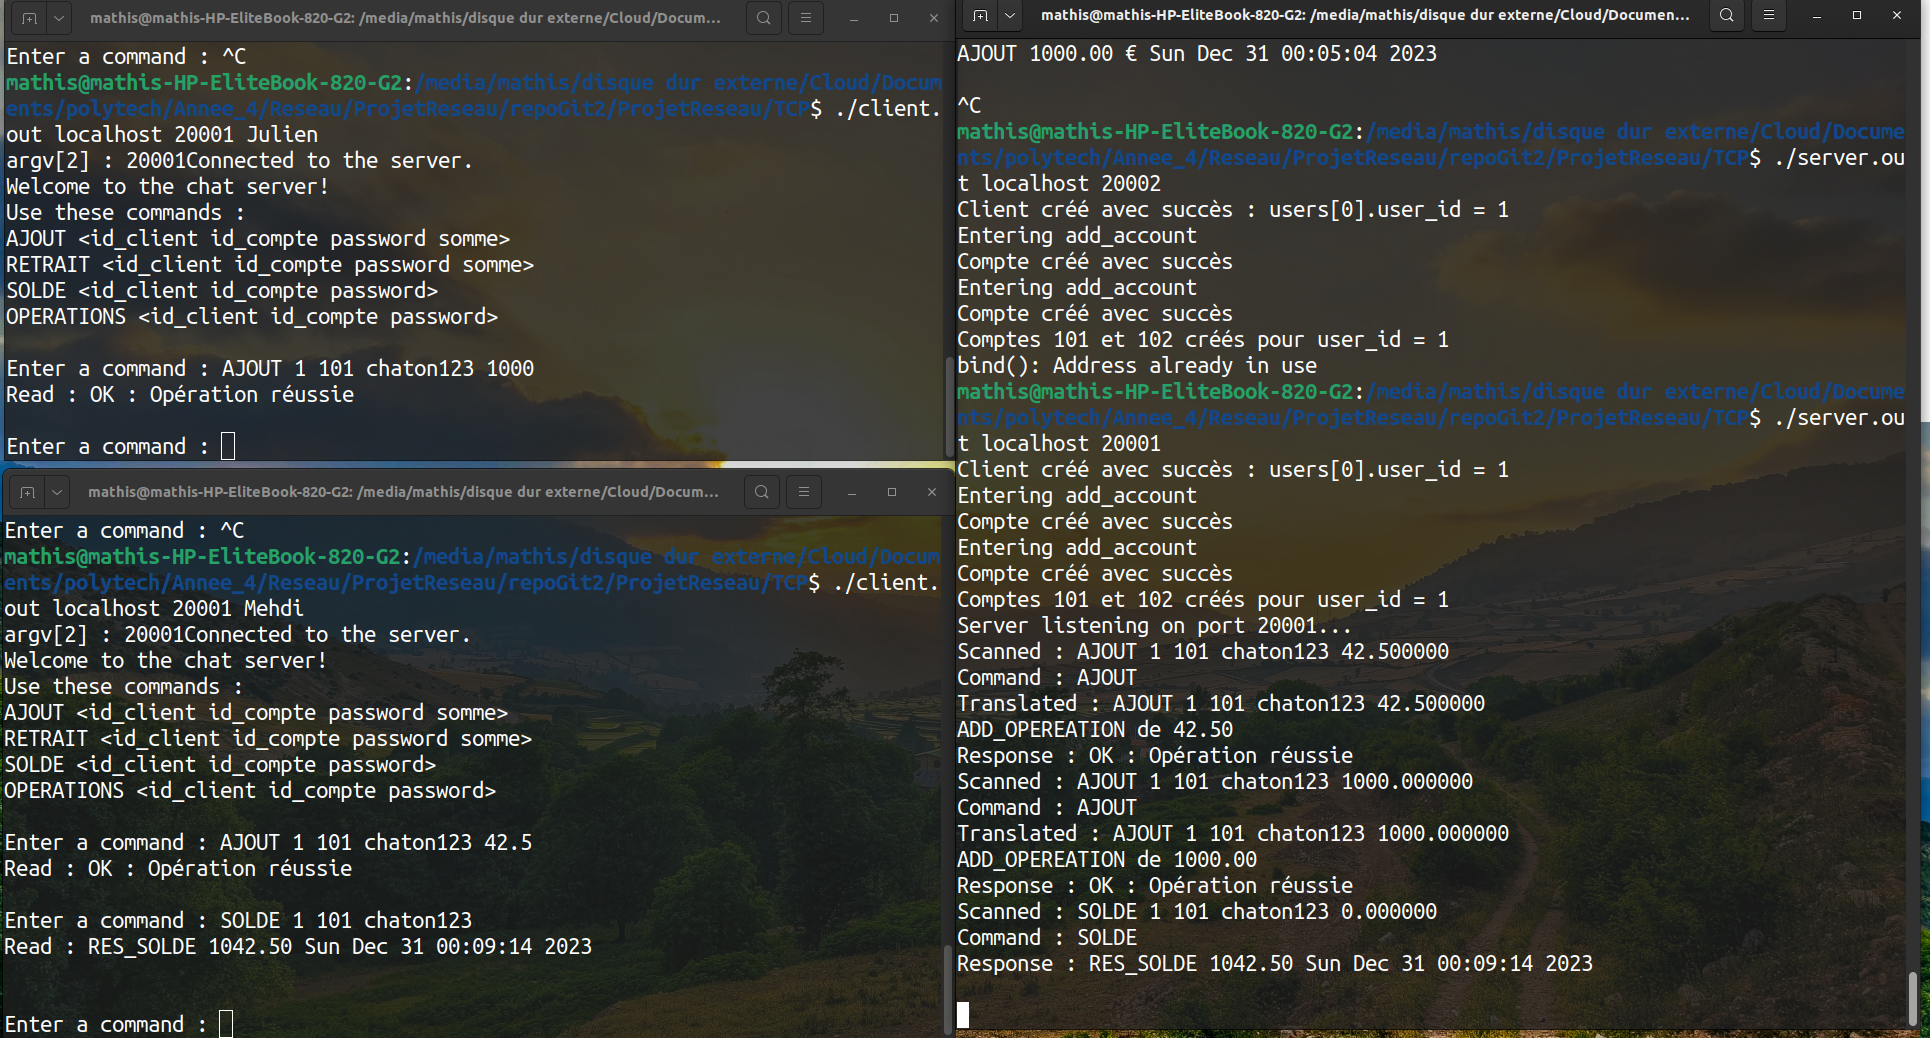
\includegraphics[width=1.25\linewidth]{TCPmultiClients.png}
    \caption{\label{fig:TCPmultiClients}Le TCP Fonctionne bien en Multi-Clients}
\end{figure}

\begin{figure}[h]
    \hspace*{-2cm}  
    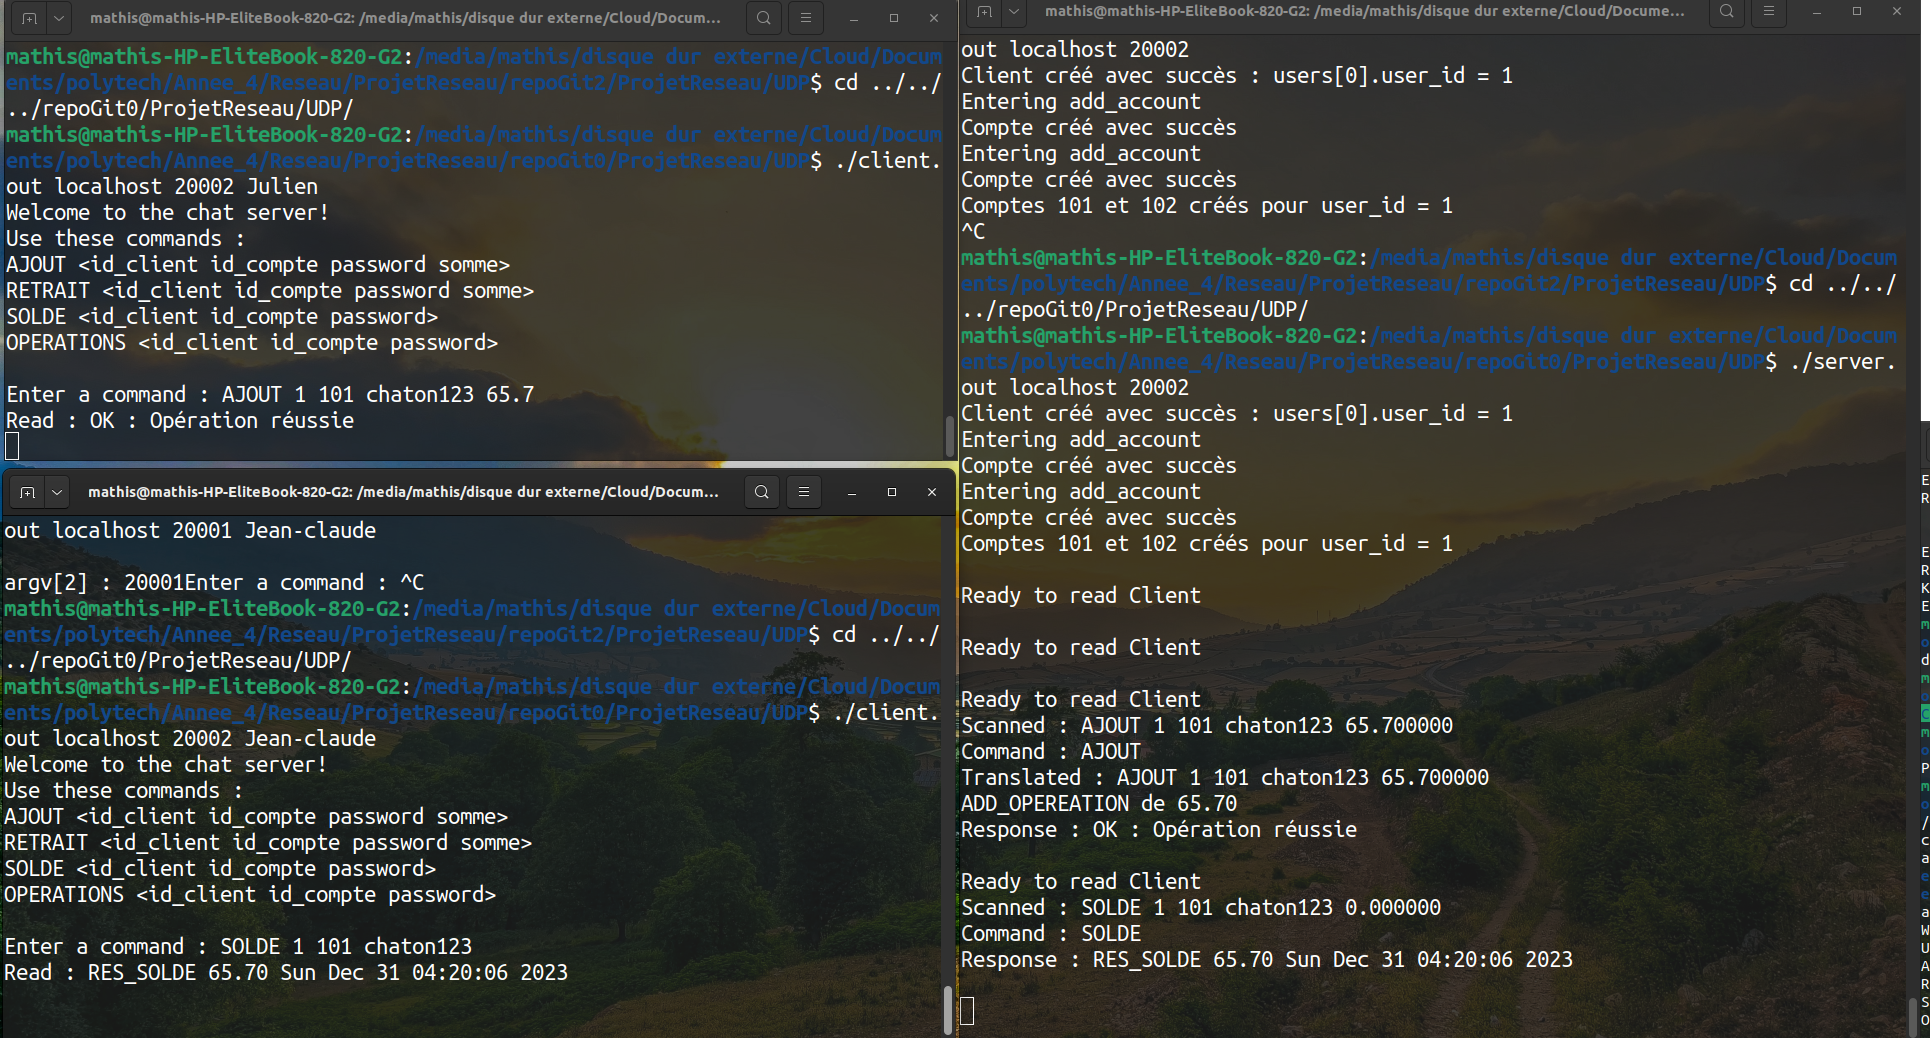
\includegraphics[width=1.25\linewidth]{UDPmultiClients.png}
    \caption{\label{fig:UDPmultiClients}Le UDP Fonctionne bien en Multi-Clients}
\end{figure}

\begin{figure}[h]
    \hspace*{-2cm}  
    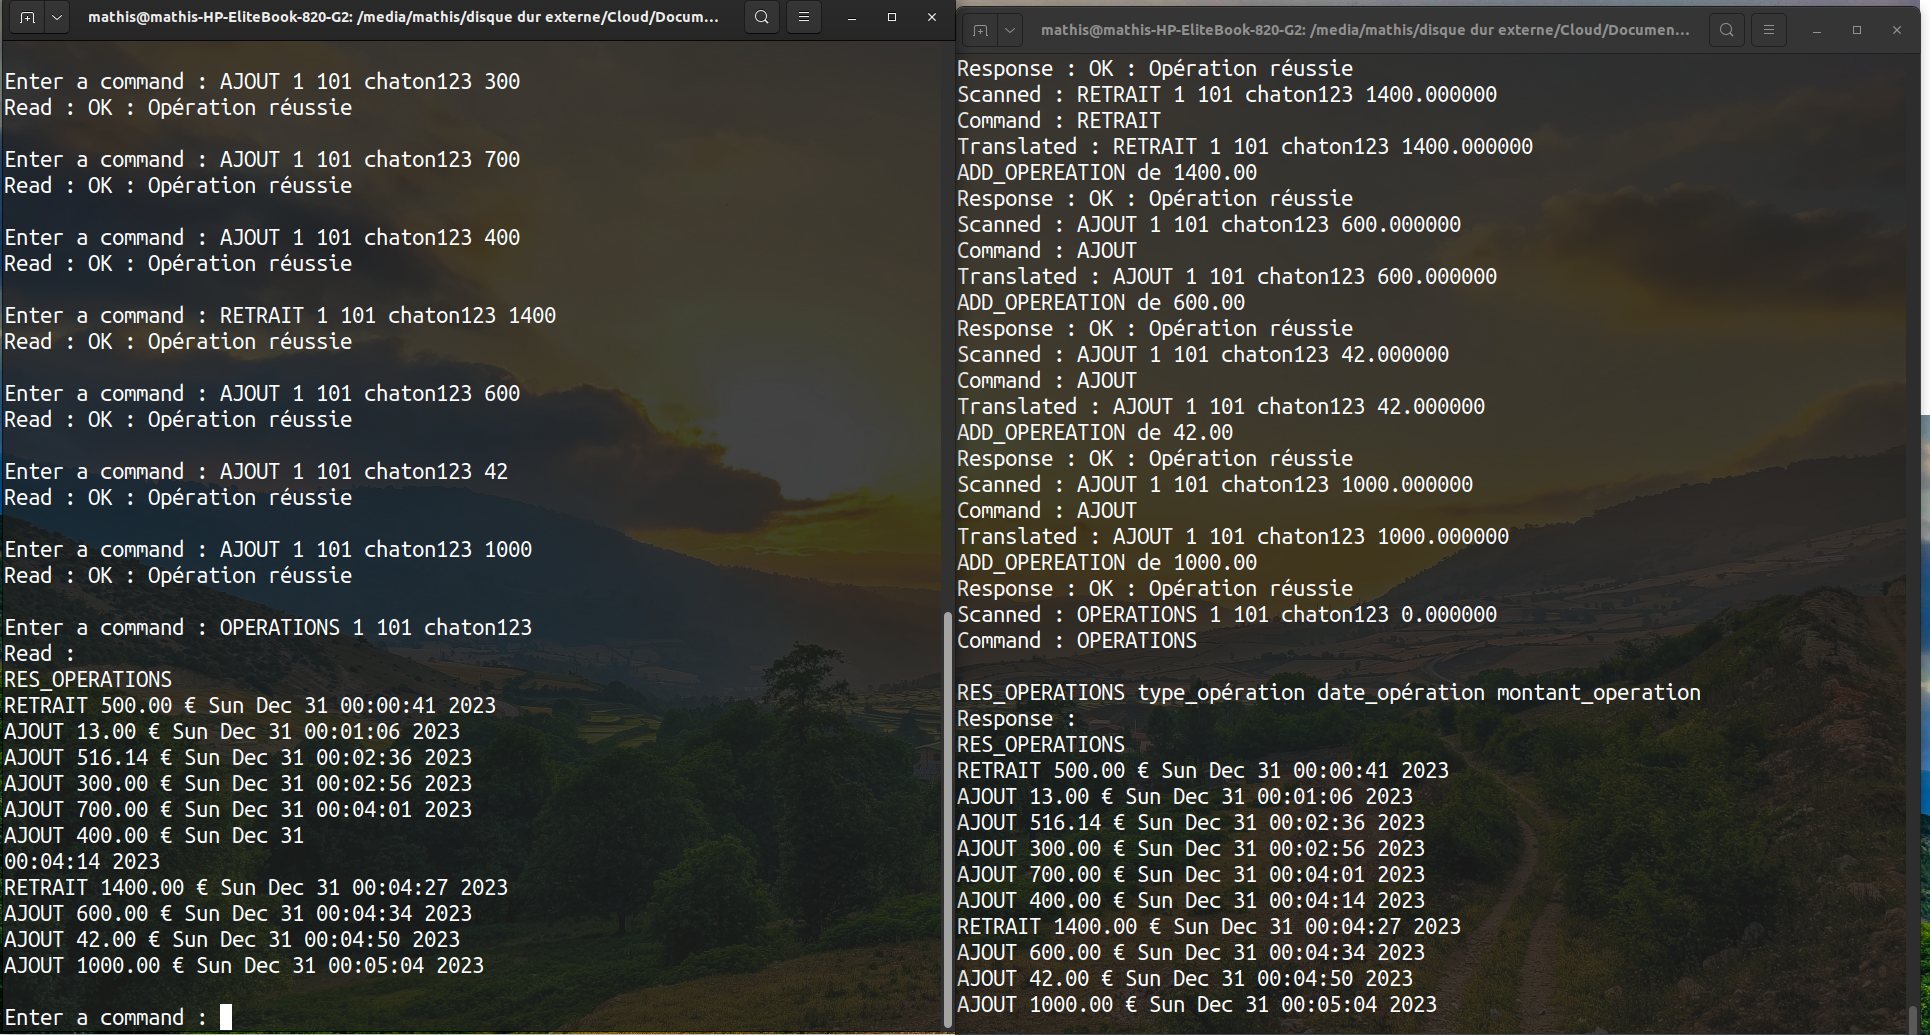
\includegraphics[width=1.25\linewidth]{OPERATIONS_TCP.png}
    \caption{\label{fig:OPERATIONS_TCP}Seulement 10 opérations s'affichent.}
\end{figure}


\end{document}

